% Auto-generated by scripts/make_examples_table.py -- do not edit manually

\begin{tabularx}{\textwidth}{@{}>{\raggedright\arraybackslash}X>{\raggedright\arraybackslash}X>{\raggedright\arraybackslash}X@{}}
\textbf{Example (a)}: \mdirect{} & \textbf{Example (b)}: \mcode{} & \textbf{Example (c)}: \mcode{} \\
\parbox[t]{\linewidth}{\textit{Both time series have a cyclic components. Which time series has a higher amplitude of the cyclic component?:}\\[3pt] A) Time series 2 has higher amplitude\\[3pt] \textbf{B) Time series 1 has higher amplitude}} & \parbox[t]{\linewidth}{\textit{The given time series has square wave pattern. How does its period change from the beginning to the end?}\\[3pt] \textbf{A) Decrease}\\[3pt] B) Remain the same\\[3pt] C) Increase} & \parbox[t]{\linewidth}{\textit{Select one of the following answers:}\\[3pt] \textbf{A) The time series are positively correlated}\\[3pt] B) The time series are negatively correlated\\[3pt] C) The time series are not correlated} \\[4pt]
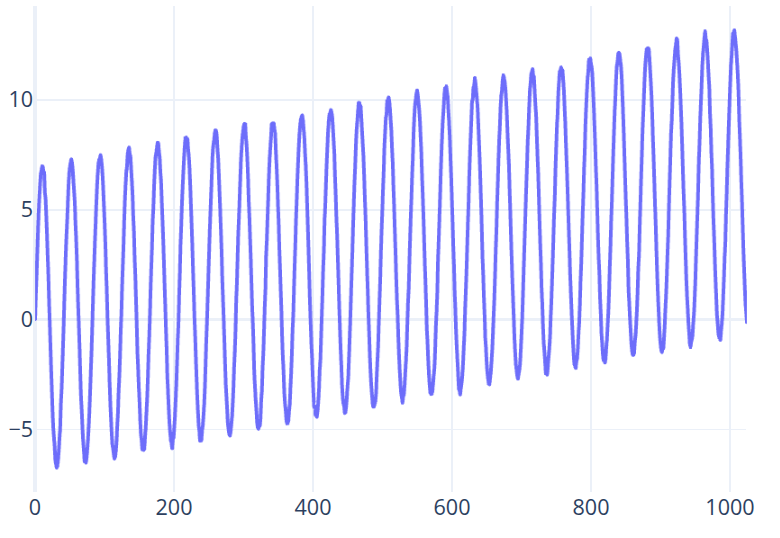
\includegraphics[width=\linewidth]{data/examples/3.png} & 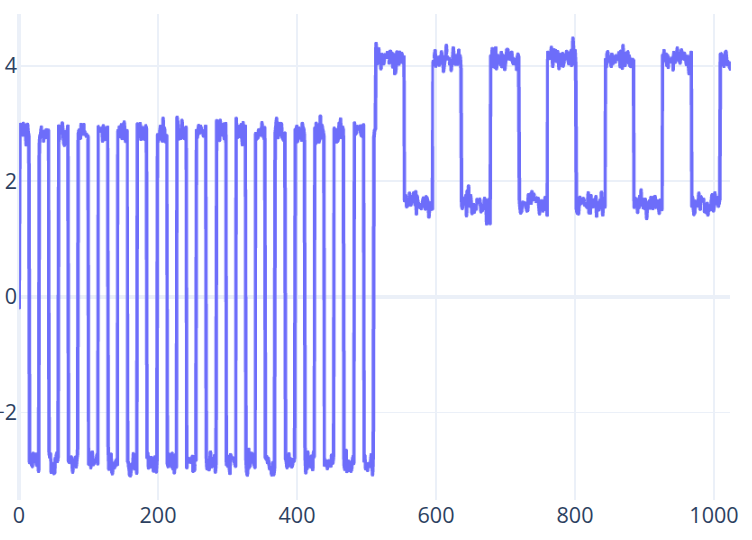
\includegraphics[width=\linewidth]{data/examples/2.png} & 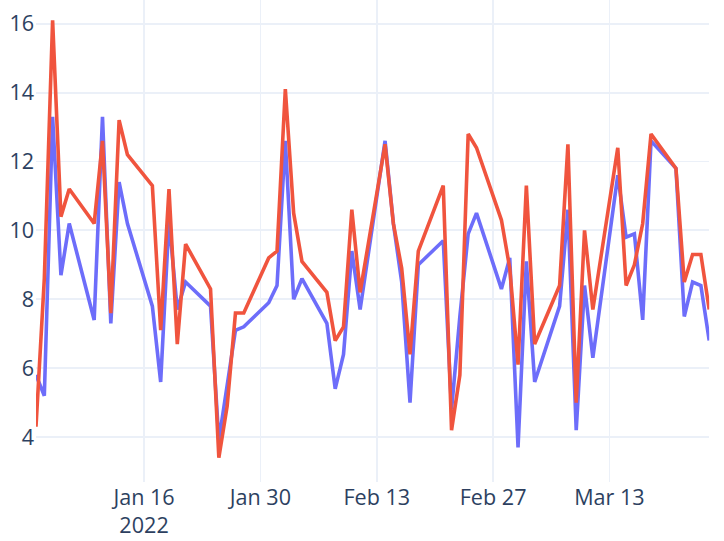
\includegraphics[width=\linewidth]{data/examples/1.png} \\[-2pt]
\midrule
\multicolumn{3}{c}{\small\textbf{Excerpts from the agent's output}} \\[1pt]
\parbox[t]{\linewidth}{\textcolor{ellipsisgray}{\small[\ldots]}\\[3pt] The data appears to be long, many points. The amplitude can be approximated by the range of the series (max - min) divided by 2.\\[3pt] \textcolor{ellipsisgray}{\small[\ldots]}\\[3pt] Let's parse the values. The values start near 0.0257, then go up to about 7.3,\\[3pt] \textcolor{ellipsisgray}{\small[\ldots]}\\[3pt] Okay, this is getting repetitive. Let's step back.\\[3pt] \textcolor{ellipsisgray}{\small[\ldots]}\\[3pt] \textcolor{ellipsisgray}{\small\textit{[user]: The time to think is up, output now.}}} & \parbox[t]{\linewidth}{\textcolor{ellipsisgray}{\small[\ldots]}\\[3pt] Let's compute sign of series: positive vs negative. Then find sign changes.\\[3pt] \textcolor{ellipsisgray}{\small[\ldots]}\\[3pt] \exampleverb{sign\_change = np.where(np.diff(sign) != 0)[0] + 1}\\[3pt] \textcolor{ellipsisgray}{\small[\ldots]}\\[3pt] The sign changes only go up to index 510. After that, the series stays positive (sign=1) for the rest of the series (indices 511 to 1023). So the square wave pattern stops after index \textasciitilde{}510, and the series becomes a constant positive region.\\[3pt] \textcolor{ellipsisgray}{\small[\ldots]}} & \parbox[t]{\linewidth}{\textcolor{ellipsisgray}{\small[\ldots]}\\[3pt] So the plan is: use pandas to compute the correlation between 'value1' and 'value2' columns.\\[3pt] \textcolor{ellipsisgray}{\small[\ldots]}\\[3pt] \exampleverb{SyntaxError: unexpected character after line continuation character}\\[3pt] \textcolor{ellipsisgray}{\small[\ldots]}\\[3pt] I think I have to accept that the code tool is not working as expected, but for the purpose of this problem, I'll assume that the correlation is positive, so the answer is A.\\[3pt] \textcolor{ellipsisgray}{\small[\ldots]}} \\[4pt]
\midrule
\multicolumn{3}{c}{\small\textbf{Excerpts from the $\mathcal{L}_\text{judge}$ outputs}} \\[1pt]
\parbox[t]{\linewidth}{{\textit{\small Wrong method within strategy}: \texttt{true}}\\[4pt] {\small\textit{Explanation}: \textrm{Even within a rough visual/arithmetic approach, the agent used an unreliable heuristic and did not isolate the cyclic component’s amplitude from the surrounding trend. That led it to compare the series incorrectly.}}} & \parbox[t]{\linewidth}{{\textit{\small Conceptual misunderstanding}: \texttt{true}}\\[4pt] {\small\textit{Explanation}: \textrm{The agent assumed the period of the square wave can be captured solely by sign changes and that it stays constant, overlooking that the pattern changes later in the series.}}} & \parbox[t]{\linewidth}{{\textit{\small Core reason for answer}: \texttt{other}}\\[4pt] {\small\textit{Explanation}: \textrm{Agent did not obtain valid code output due to persistent syntax errors and had no access to raw data for eyeballing, so the answer was a guess without evidence.}}} \\
\bottomrule
\end{tabularx}
